\subsubsection{Scheduling basato sullo stato energetico dei nodi}
\label{subsubsec:node_energy_scheduling}

Una prima tipologia di scheduler energeticamente consapevoli considera
l'energia come proprietà dei nodi dell'infrastruttura, utilizzando lo
stato energetico corrente come criterio primario per le decisioni di
\emph{placement}. In questo paradigma, le invocazioni vengono
redistribuite tra nodi con diversa disponibilità energetica al fine di
preservare la continuità operativa dell'infrastruttura nel suo complesso.

Tale approccio è particolarmente rilevante in scenari di Edge Computing
distribuito, nei quali i nodi possono essere alimentati da fonti
rinnovabili intermittenti e presentare livelli di carica variabili nel
tempo. In questi contesti, l'obiettivo dello scheduler non è la
minimizzazione del consumo medio, bensì il mantenimento
dell'operatività dell'intero sistema, evitando che nodi con
disponibilità energetica ridotta diventino temporaneamente
irraggiungibili.

Un esempio rappresentativo di questo approccio è il sistema
\emph{Faashouse}~\cite{faashouse}, progettato per ambienti serverless
all'estremo edge. Come illustrato in
Figura~\ref{fig:faashouse_architecture}, l'architettura si articola su
più livelli: dispositivi edge a bassa potenza, piattaforma di
containerizzazione e orchestrazione, e livello serverless per la
gestione delle funzioni.

\begin{figure}[ht]
    \centering
    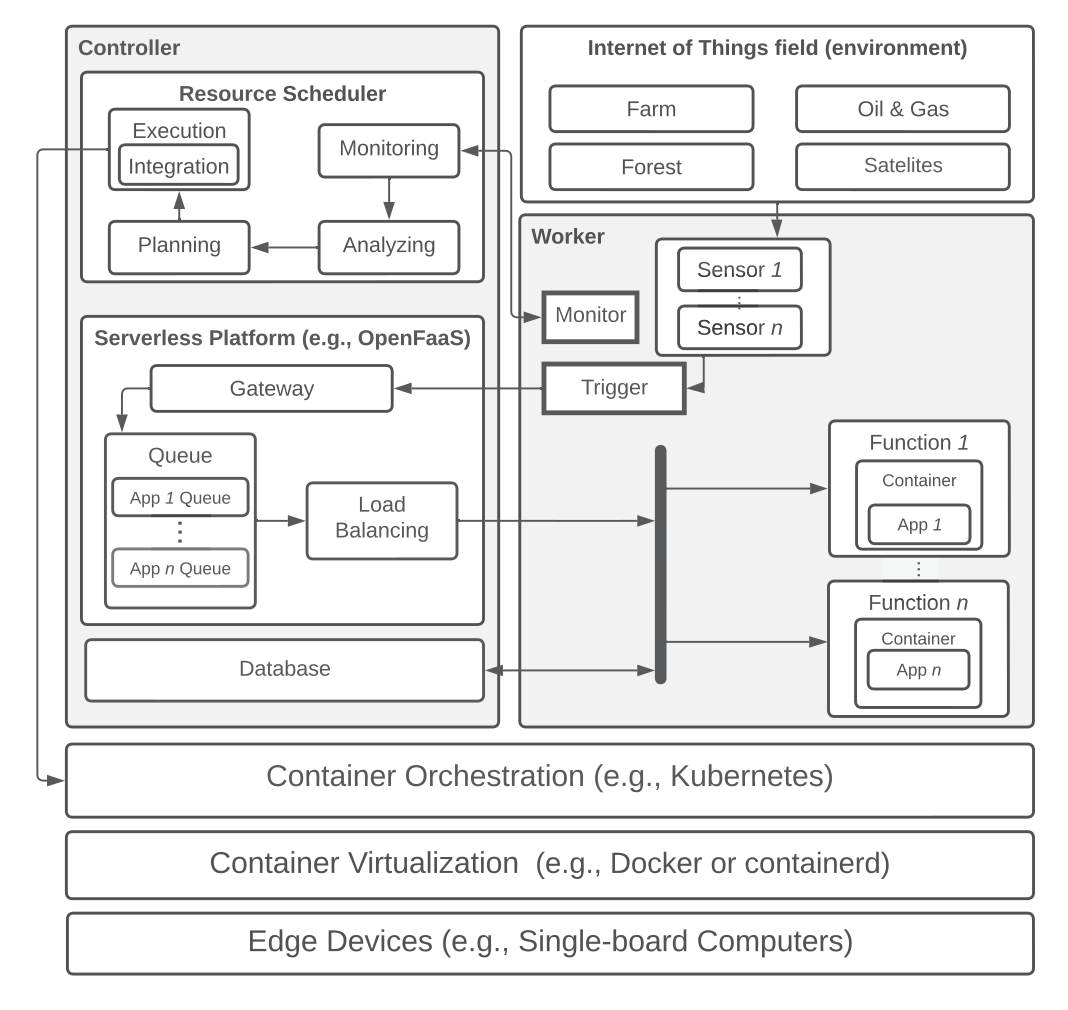
\includegraphics[width=0.9\textwidth]{figures/FaasHouse.png}
    \caption{Architettura del sistema Faashouse. Il controller integra un
    \emph{Resource Scheduler} che, seguendo un ciclo di monitoraggio,
    analisi e pianificazione, decide il \emph{placement} delle funzioni
    sui nodi worker in base allo stato energetico corrente.}
    \label{fig:faashouse_architecture}
\end{figure}

Il \emph{Resource Scheduler}, ospitato nel controller, implementa un
ciclo di controllo riconducibile al modello MAPE (\emph{Monitoring,
Analyzing, Planning, Execution}): monitora continuamente lo stato dei
nodi, analizza le condizioni operative correnti, pianifica le decisioni
di \emph{placement} e le applica all'infrastruttura. Il parametro
decisionale principale è il livello di carica dei nodi (\emph{State of
Charge}, SoC), che riflette la disponibilità energetica residua di
ciascun elemento dell'infrastruttura.

Dal punto di vista modellistico, lo stato energetico di ciascun nodo è
una grandezza variabile nel tempo, determinata congiuntamente
dall'energia dissipata durante l'esecuzione delle funzioni e
dall'eventuale energia generata localmente. Le decisioni di assegnazione
incidono direttamente sull'evoluzione di tale stato: concentrare le
invocazioni su nodi con SoC ridotto può comprometterne la disponibilità
futura, mentre una redistribuzione bilanciata consente di preservare
l'operatività dell'intero sistema. Quando il livello di carica di un
nodo si avvicina a una soglia critica, le nuove richieste vengono
reindirizzate verso nodi più stabili mediante meccanismi di offloading,
realizzando un bilanciamento energetico dinamico.

È opportuno sottolineare che Faashouse opera a granularità di nodo e
non di funzione: le invocazioni sono trattate come unità indivisibili e
non sono previste varianti della stessa funzione con profili energetici
differenziati. L'ottimizzazione si realizza esclusivamente attraverso
la selezione del nodo di esecuzione, senza intervenire sulla logica
applicativa. Questa scelta progettuale delimita l'ambito di applicabilità
del sistema: in scenari in cui il consumo energetico per invocazione
dipende dalla complessità computazionale della funzione, la sola
redistribuzione del carico potrebbe risultare insufficiente per
soddisfare vincoli energetici stringenti a livello di singola esecuzione.